
\documentclass[runningheads, a4paper, oribibl]{llncs}

\setcounter{tocdepth}{3}
\usepackage{graphicx}
\graphicspath{{../images/}}
\usepackage{epstopdf}
\usepackage{standalone}
\usepackage{xcolor}
\usepackage{tikz}
\usetikzlibrary{fit}
\usetikzlibrary{shapes,snakes,calc}



\usepackage{listings, color}

\definecolor{dkgreen}{rgb}{0,0.6,0}
\definecolor{gray}{rgb}{0.5,0.5,0.5}
\definecolor{mauve}{rgb}{0.58,0,0.82}



\lstset{frame=tb,
  language=Matlab,
  aboveskip=3mm,
  belowskip=3mm,
  showstringspaces=false,
  columns=flexible,
  basicstyle={\small\ttfamily},
  numbers=none,
  numberstyle=\tiny\color{gray},
  keywordstyle=\color{blue},
  commentstyle=\color{dkgreen},
  stringstyle=\color{mauve},
  breaklines=true,
  breakatwhitespace=false,
  tabsize=2,
  numbers=left,
  numbersep=5pt,
  title=\lstname
}



\usepackage[section]{placeins}

\usepackage{amsmath,amssymb, cancel}
%



\renewcommand\thesubsection{\thesection(\alph{subsection})}


\begin{document}

\mainmatter

\title{High Performance Computing Report\\Lab 5}

\titlerunning{High Performance Computing Report}

\author{Amarnath Karthi (201501005)\\Chahak Mehta (201501422)}%
%
\authorrunning{Amarnath Karthi \& Chahak Mehta}
\institute{DA-IICT\\
  \mailsa\\
  \mailsb\\
}

\maketitle


\section{Image warping}
\begin{figure}[h!]
    \centering
    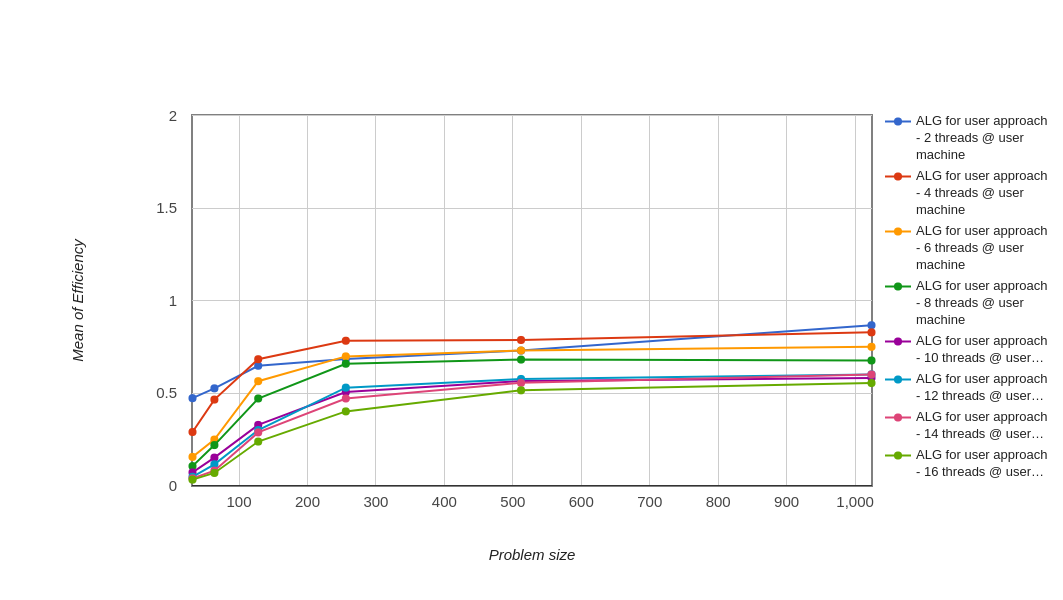
\includegraphics[scale = 0.3]{q1/mean_efficiency.png}
    \caption{Efficiency vs problem size}
    \label{fig:q1_eff}
\end{figure}

\begin{figure}[h!]
    \centering
    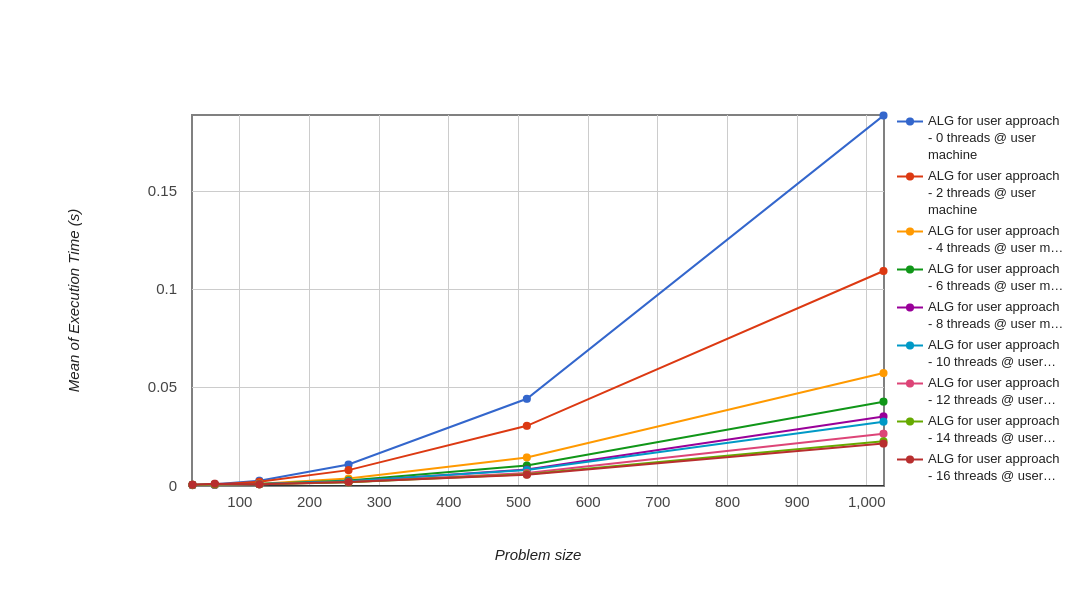
\includegraphics[scale = 0.3]{q1/mean_executionTime.png}
    \caption{Execution time vs problem size}
    \label{fig:q1_time}
\end{figure}

\begin{figure}[h!]
    \centering
    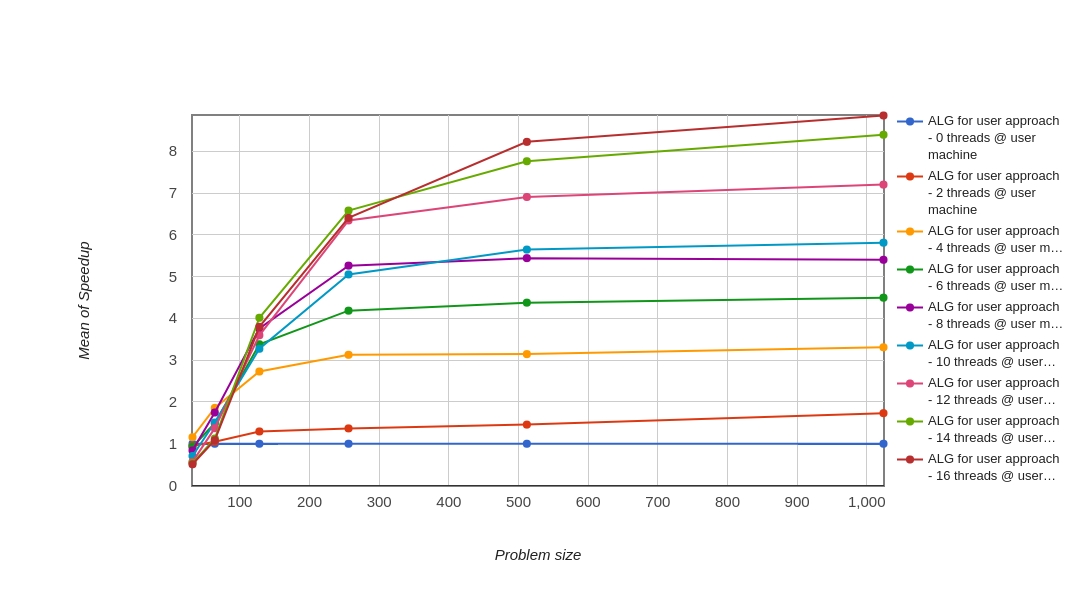
\includegraphics[scale = 0.3]{q1/mean_speedup.png}
    \caption{Speedup vs problem size}
    \label{fig:q1_speedup}
\end{figure}


\textbf{Implementation Details}
\subsection{Brief and clear description about the Serial implementation}
The test image is warped by using the principle of rotation and changing the angle of rotation (theta) according to the number of pixels/distance.

\subsection{Brief and clear description about the implementation of the approach (Parallelization Strategy, Mapping of computation to threads)}
The serial code is then parallelized by using OpenMP parallel directive and by manually assigning the threads the chunks of the image the thread has to work on thereby working on the principle of data division

\subsection{Time Curve related analysis (as no. of processor increases)}
We can see from Figure \ref{fig:q1_eff} that the time taken by the parallel program to run decreases as the number of cores that perform the operations. This is due to the division of the work to be done among more number of available cores which in turn leads to more parallel operations to be performed, thereby decreasing the execution time for the code.

\subsection{Time Curve related analysis (as problem size increases, also for serial)}
As the problem size increases, the time taken by the serial code increases exponentially. The time taken by the parallel code increases at a much slower rate because of the reasons mentioned in the above answer.

\subsection{Speedup Curve related analysis (as problem size and no. of processors increase)}
We can see in the Speedup curve that the parallel  code is faster by a factor of maximum 9, unlike the theoretical factor of 16. This is due to the increase in the parallel overhead with the increase in the number of threads/processors performing the operations

\subsection{Efficiency Curve related analysis}
The efficiency for cores can be calculated by $\frac{speedup}{number of processors}$ This doesn't reach 1 because of the fact that the speedup is much lower than the theoretical value of the speedup for a particular number of cores

\section{Image median filtering}
\begin{figure}[h!]
    \centering
    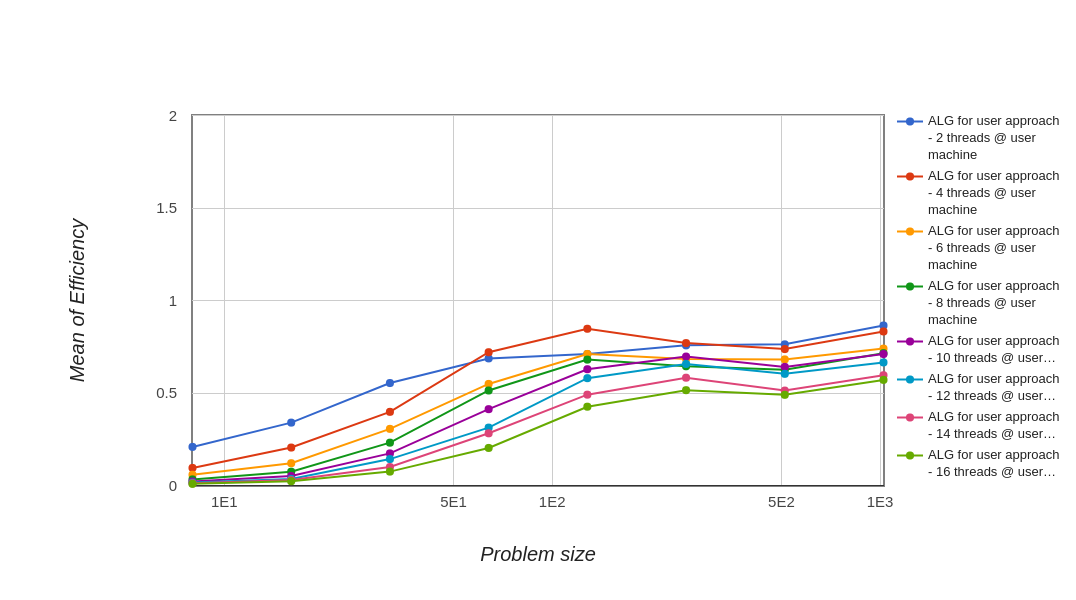
\includegraphics[scale = 0.3]{q2/mean_efficiency.png}
    \caption{Efficiency vs problem size}
    \label{fig:q2_eff}
\end{figure}

\begin{figure}[h!]
    \centering
    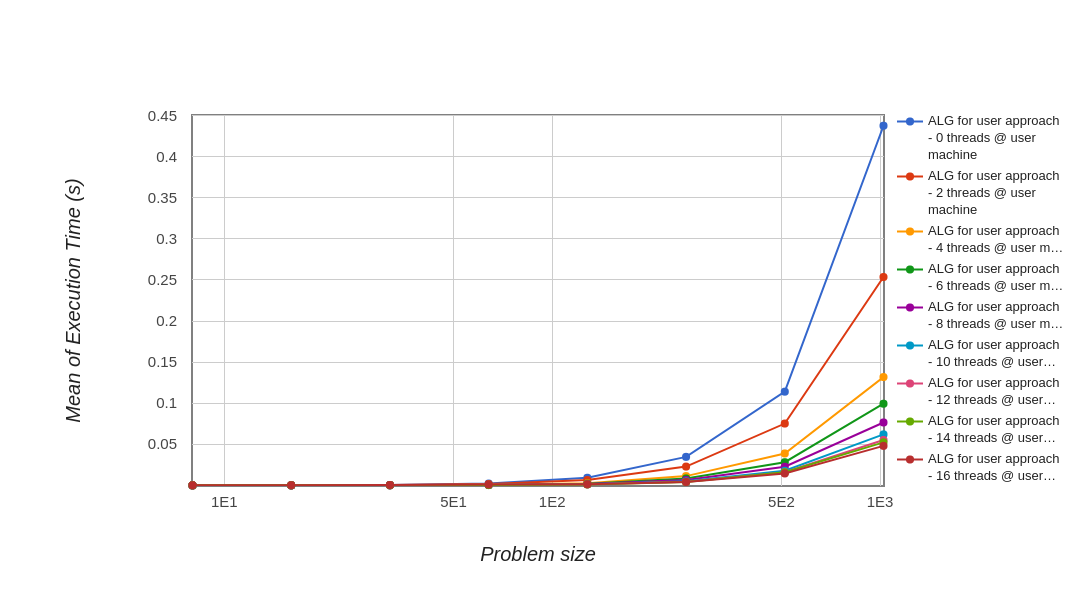
\includegraphics[scale = 0.3]{q2/mean_executionTime.png}
    \caption{Execution time vs problem size}
    \label{fig:q2_time}
\end{figure}

\begin{figure}[h!]
    \centering
    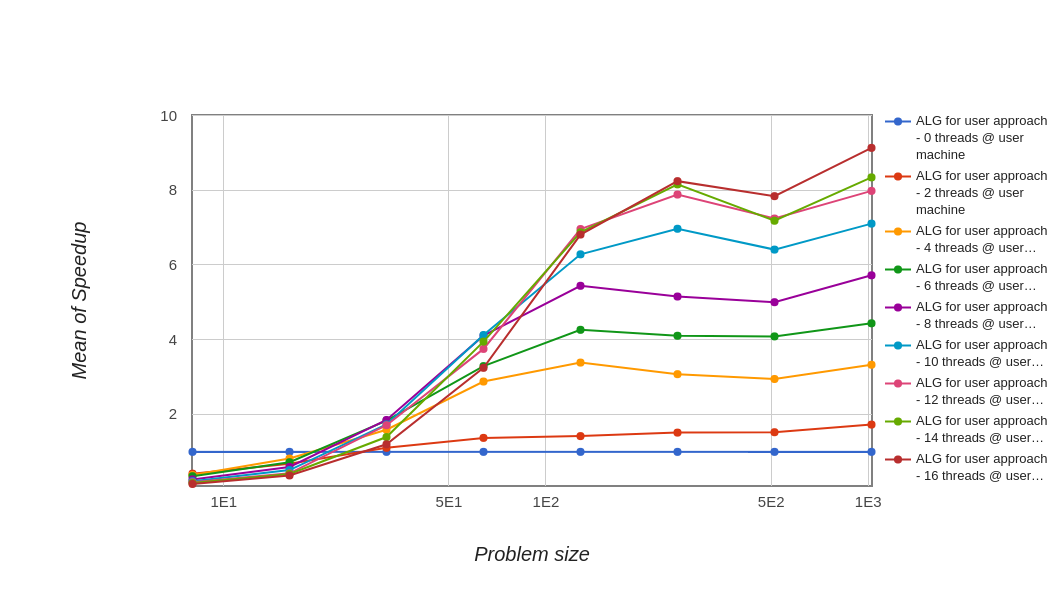
\includegraphics[scale = 0.3]{q2/mean_speedup.png}
    \caption{Speedup vs problem size}
    \label{fig:q2_speedup}
\end{figure}


\textbf{Implementation Details}
\subsection{Brief and clear description about the Serial implementation}
The test image is filtered using the concept of median filtering. For this, the data values of the pixels are determined by the median of the values of the pixels in the neighbourhood of a specified halfwidth. Increasing the size of the halfwidth will increas the time taken to run the code since it increases the number of pixels to be taken into account to determine the median of a neighbourhood of a pixel which will slow down the code considerably.(This technique can also be used to filter out noise from noisy images or as an enhancement filter on other images).

\subsection{Brief and clear description about the implementation of the approach (Parallelization Strategy, Mapping of computation to threads)}
The serial code is parallelized by using OpenMP parallel directive and by manually assigning the threads the chunks of the image the thread has to work on thereby working on the principle of data division

\subsection{Time Curve related analysis (as no. of processor increases)}
We can see from Figure \ref{fig:q2_eff} that the time taken by the parallel program to run decreases as the number of cores that perform the operations. This is due to the division of the work to be done among more number of available cores which in turn leads to more parallel operations to be performed, thereby decreasing the execution time for the code.

\subsection{Time Curve related analysis (as problem size increases, also for serial)}
As the problem size increases, the time taken by the serial code increases exponentially. The time taken by the parallel code increases at a much slower rate because of the reasons mentioned in the above answer.

\subsection{Speedup Curve related analysis (as problem size and no. of processors increase)}
We can see in the Speedup curve that the parallel  code is faster by a factor of maximum 9, unlike the theoretical factor of 16. This is due to the increase in the parallel overhead with the increase in the number of threads/processors performing the operations

\subsection{Efficiency Curve related analysis}
The efficiency for cores can be calculated by $\frac{speedup}{number of processors}$ This doesn't reach 1 because of the fact that the speedup is much lower than the theoretical value of the speedup for a particular number of cores
\section{Image normalization}
\begin{figure}[h!]
    \centering
    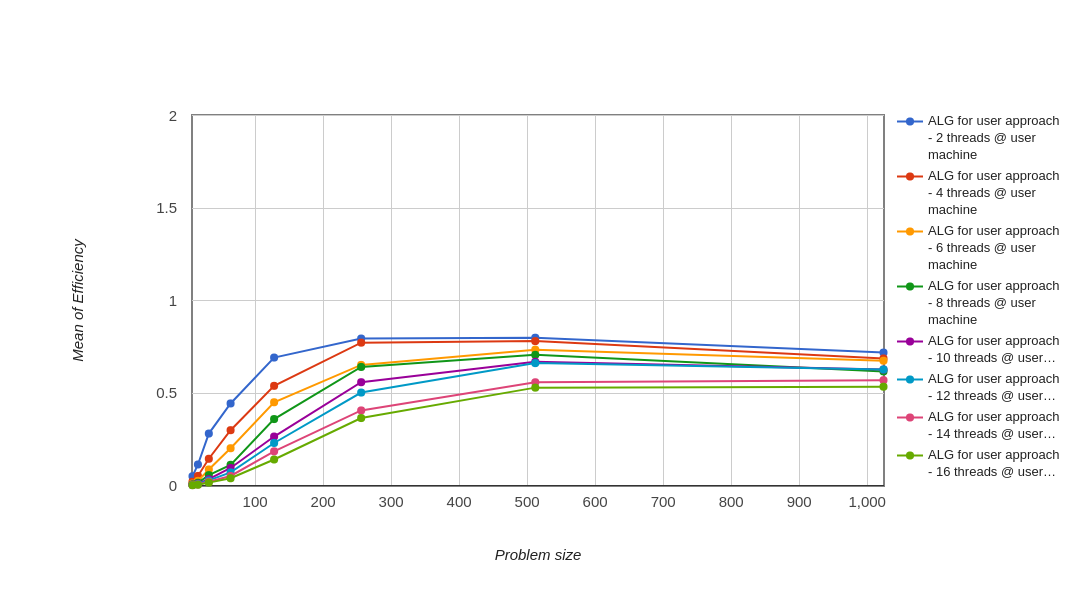
\includegraphics[scale = 0.3]{q3/mean_efficiency.png}
    \caption{Efficiency vs problem size}
    \label{fig:q3_eff}
\end{figure}

\begin{figure}[h!]
    \centering
    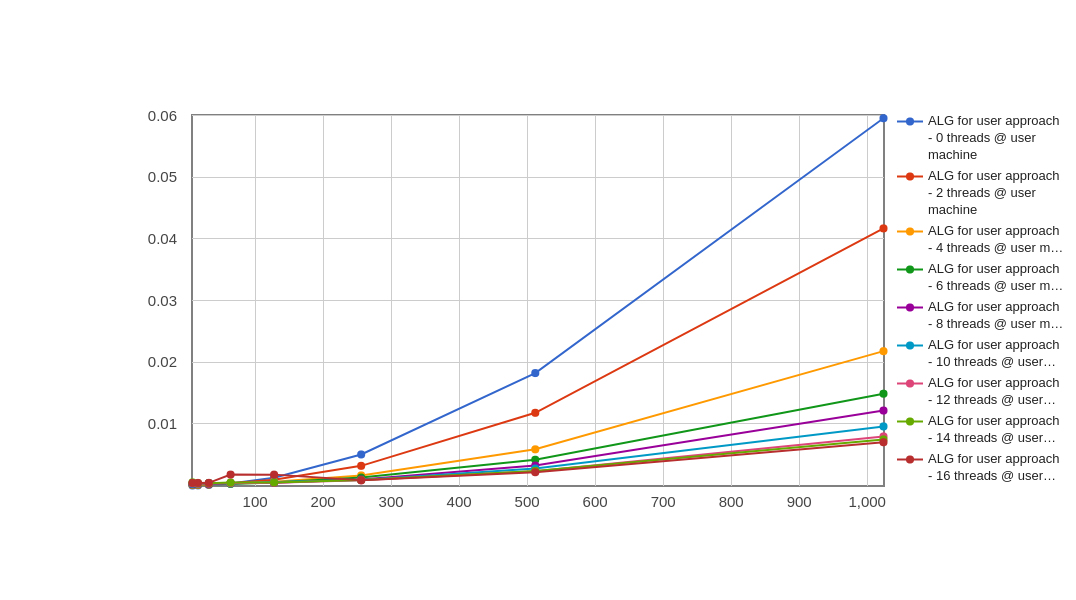
\includegraphics[scale = 0.3]{q3/mean_executionTime.png}
    \caption{Execution time vs problem size}
    \label{fig:q3_time}
\end{figure}

\begin{figure}[h!]
    \centering
    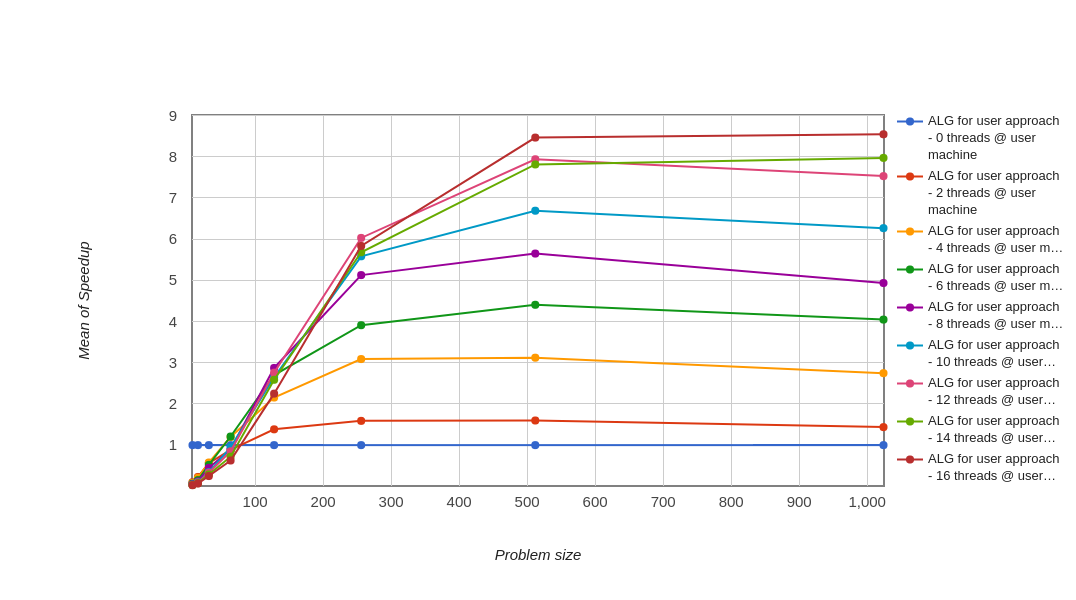
\includegraphics[scale = 0.3]{q3/mean_speedup.png}
    \caption{Speedup vs problem size}
    \label{fig:q3_speedup}
\end{figure}


\textbf{Implementation Details}
\subsection{Brief and clear description about the Serial implementation}
The test image is normalized by using the formula to standardize a Gaussian variable. This is done by calculating the Mean and Standard deviation of the values of the pixels of the image and then by the formula $Z=\frac{X-\mu}{\sigma}$.

\subsection{Brief and clear description about the implementation of the approach (Parallelization Strategy, Mapping of computation to threads)}
The serial code is then parallelized by using OpenMP parallel directive and by manually assigning the threads the chunks of the image the thread has to work on thereby working on the principle of data division

\subsection{Time Curve related analysis (as no. of processor increases)}
We can see from Figure \ref{fig:q3_eff} that the time taken by the parallel program to run decreases as the number of cores that perform the operations. This is due to the division of the work to be done among more number of available cores which in turn leads to more parallel operations to be performed, thereby decreasing the execution time for the code.

\subsection{Time Curve related analysis (as problem size increases, also for serial)}
As the problem size increases, the time taken by the serial code increases exponentially. The time taken by the parallel code increases at a much slower rate because of the reasons mentioned in the above answer.

\subsection{Speedup Curve related analysis (as problem size and no. of processors increase)}
We can see in the Speedup curve that the parallel  code is faster by a factor of maximum 9, unlike the theoretical factor of 16. This is due to the increase in the parallel overhead with the increase in the number of threads/processors performing the operations

\subsection{Efficiency Curve related analysis}
The efficiency for cores can be calculated by $\frac{speedup}{number of processors}$ This doesn't reach 1 because of the fact that the speedup is much lower than the theoretical value of the speedup for a particular number of cores

\section{Additional Image Results}

\begin{figure}[h!]
    \centering
    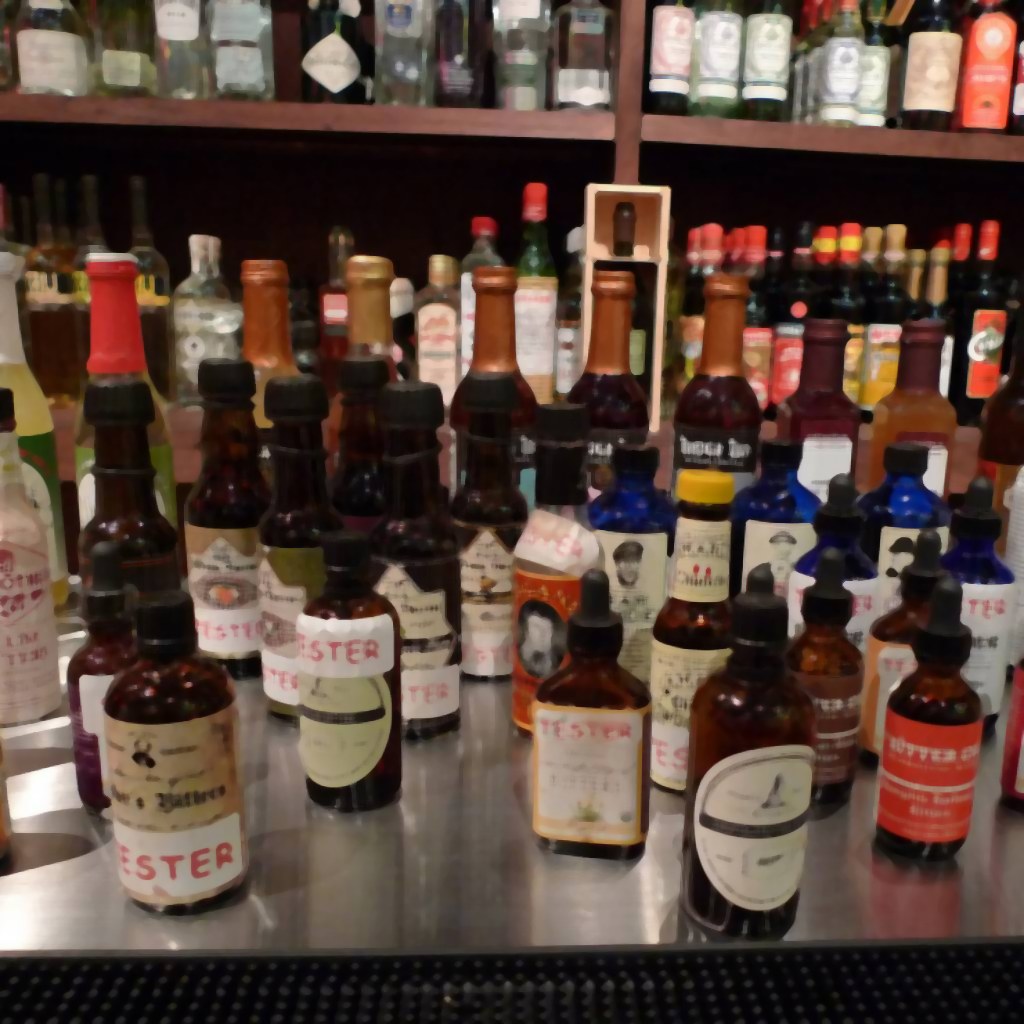
\includegraphics[scale = 0.4]{q1/1024.png}
    \caption{Median filtering on an image of resolution 1024x1024}
    \label{fig:1}
\end{figure}

\begin{figure}[h!]
    \centering
    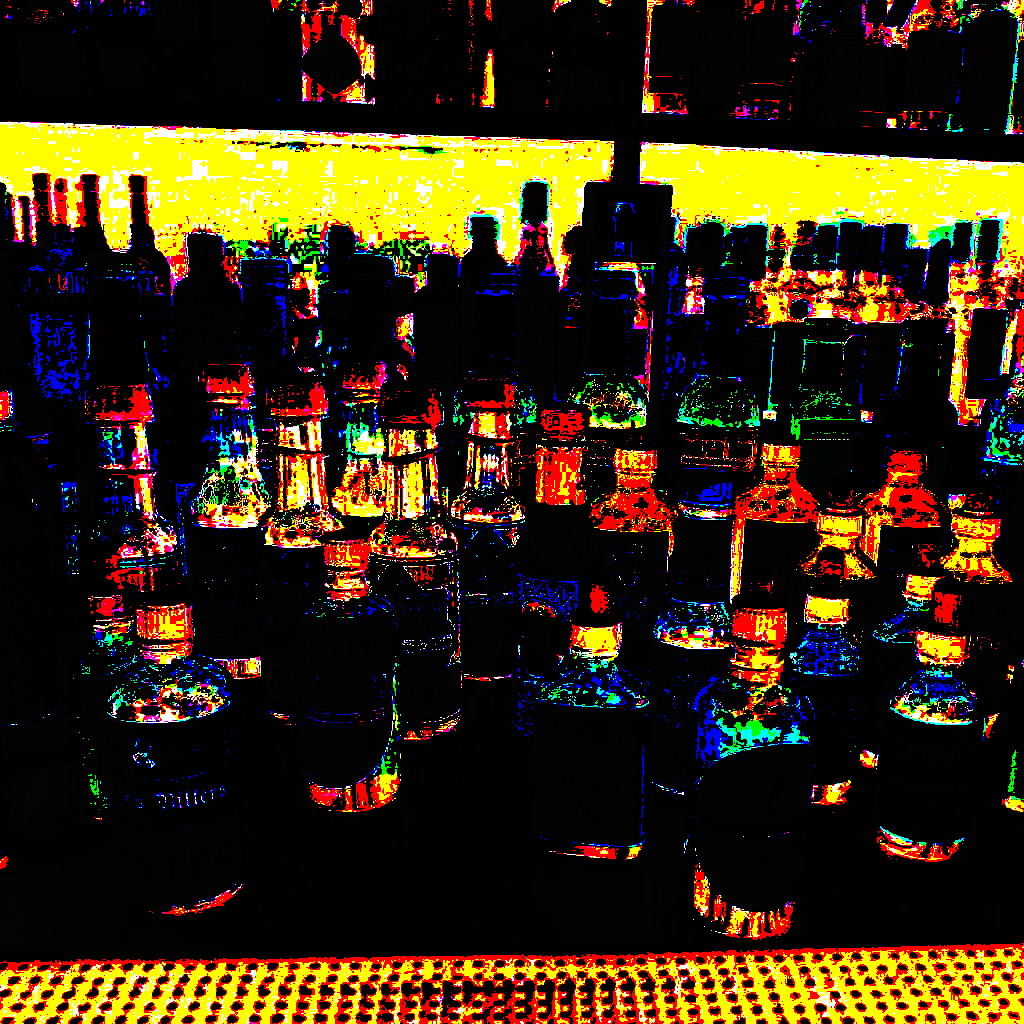
\includegraphics[scale = 0.4]{q1/norm.png}
    \caption{Normalisation on an image of resolution 1024x1024}
    \label{fig:2}
\end{figure}

\end{document}
